\lab{Predator-Prey and Weight Change Models}{Weight change and Predator-Prey Models}
\label{lab:Weightchange}
\objective{We introduce built-in methods for solving Initial Value Problems and apply the methods to two dynamical systems.
The first  system looks at the relationship between a predator and its prey. 
The second model is a weight change model based on thermodynamics and kinematics.}

\section*{ODE Solvers}
Initial Value Problems (IVPs) are a systems of one or more ordinary differential equations (ODEs) with defined initial conditions. In some cases, these can be solved by hand, but in real life it is more practical to use numerical solvers. For this lab you will use the  \li{solve_ivp} solver from the \li{scipy.integrate} library.

\li{solve_ivp} solves a system of ODEs given by $dy/dt = f(t, y),\quad y(t_0)=y_0$, where $y$ can be a vector. The solver takes as parameters the callable function $f$, the time boundaries \li{(t0,tf)}, the initial condition \li{y_0}, and an optional keyword argument \li{t_eval} that designates the times at which the solver will store the solution. Then \li{solve_ivp} returns a bunch object containing an array \li{y} with shape \li{(len(y_0), len(t))}, where each column gives the \li{y} values for one time point. The syntax for \li{solve_ivp} is shown below.
\begin{lstlisting}
from scipy.integrate import solve_ivp
sol = solve_ivp(f, (t0,tf), y0, t_eval=t)
\end{lstlisting}
Assuming that $f$, $y0$, $t_0$, $t_f$, and $t$ are previously defined as explained above, \li{sol.y} is a vector containing the solution to the IVP and can be visualized by plotting each row of \li{sol.y} against the time domain or by plotting the rows against each other.

\section*{Predator-Prey Model} 
ODEs are commonly used to model relationships between predator and prey populations. For example, consider the populations of wolves, the predator, and rabbits, the prey), in Yellowstone National Park. Let $r(t)$ and $w(t)$ represent the rabbit and wolf populations respectively at time $t$, measured in years. 
We will make a few assumptions to simplify our model:

\begin{itemize}
\item In the absence of wolves, the rabbit population grows at a positive rate proportional to the current population. Thus when $w(t) = 0$, $dr/dt = \alpha r(t)$, where $\alpha > 0$.
\item In the absence of rabbits, the wolves die out. Thus when $r(t) = 0$, $dw/dt = -\delta w(t)$, where $\delta > 0$.
\item The number of encounters between rabbits and wolves is proportional to the product of their populations. The wolf population grows proportional to the number of encounters by $\beta r(t)w(t)$ (where $\beta > 0$), and the rabbit population decreases proportional to the number of encounters by $-\gamma r(t)w(t)$ (where $\gamma > 0$). 
\end{itemize}

This leads to the following system of ODEs: 
\begin{align}
	\begin{split}
	&\frac{dr}{dt} = \alpha r - \beta r w = r(\alpha - \beta w)\\
	&\frac{dw}{dt} = -\delta w + \gamma r w = w(-\delta + \gamma r)
	\end{split}\label{eqn: Pred-Prey}
\end{align}

\begin{figure}
\centering
\includegraphics[width=\textwidth]{figures/Predator_Prey.png}
\caption{The solution to the system found in \eqref{eqn: Pred-Prey}}
\label{fig: Pred-Prey}
\end{figure}



\begin{problem}
As mentioned above, the \li{solve_ivp} solver requires a callable function representing the right hand side of the IVP. 
Define the function \li{predator_prey()} that accepts the current $r(t)$ and $w(t)$ values as a 1d array $y$, and the current time $t$, 
%a 1d array $y$ representing the current rabbit and wolf populations and a float $t$ representing the current time. 
and returns the right hand side of \eqref{eqn: Pred-Prey} as an ndarray. 
Use $\alpha=1.0$, $\beta=0.5$, $\delta=0.75$, and $\gamma=0.25$ as your growth parameters.
%\begin{lstlisting}
%def predator_prey(y, t):
%	'''
%	Parameters:
%	--------------
%	t:	time variable.
%	y:	an array of length len(y0) representing current wolf and rabbit populations at time t.
%	
%	Return:
%	--------
%	Return a tuple corresponding to the Predator-Prey model.
%	'''
%	pass
%\end{lstlisting}

\end{problem}

%Import the \li{odeint} method and define the initial conditions and time array for the predator-prey model using the following code:
%\begin{lstlisting}
%# Initialize populations
%r0 = 5
%w0 = 3
%y0 = [r0, w0]

%# Initialize time array
%t = np.linspace(0, 20, 100)
%\end{lstlisting}

\begin{problem}
Use \li{solve_ivp} to solve \eqref{eqn: Pred-Prey} with initial conditions $(r_0, w_0) = (5, 3)$ and time ranging from $0$ to $20$ years.
Display the resulting rabbit and wolf populations over time (stored as rows in the attribute \li{y} of the output of \li{solve_ivp}) on the same plot. Your graph should match the graph in figure \ref{fig: Pred-Prey}.
\end{problem}

\begin{comment}
\objective{We use IVP methods to study two dynamical systems. 
The first  system is a weight change model based on thermodynamics and kinematics. 
The second model looks at the relationship between a predator and its prey. }

\section*{ODE solvers}
Initial Value Problems, or IVPs, are a system of one or more ordinary differential equations (ODEs) with initial values.
In more basic math courses, these problems can be solved by hand, but in real life that is very much not the case.
For more complicated IVPs, numerical solvers are required.

In the previous lab, you built your own numerical solvers. For this lab you will use two built in solvers from the \li{scipy.integrate} library, \li{ode} and \li{odeint}. The \li{ode} solver solves a single equation of the form $u'(t)=f(t,u)$ and takes the function $f$ as a parameter. This solver can be implemented with various numerical approximations. We will use the \li{dopri5} method, which runs RK4 iterative ODE solver (Runge-Kutta method of order 4). The \li{odeint} solver is similar but solves a system of ODEs rather than a single equation.

In later labs we will build our own numerical solvers but for this lab you will learn how to use two methods built in to Python. You will be expected to use these methods to solve ODEs in future labs.

The solvers used in this lab are contained in the \li{scipy.integrate} library. The first solver, \li{scipy.integrate.ode}, solves the equation $u'(t)=f(t,u)$ and takes the function $f$ as a parameter. 

The \li{ode} method can use many numerical approximations to solve.
We will use the \li{dopri5} method, which runs the RK4 (Runge-Kutta method of order 4) iterative ODE solver.

At the end of this lab you will see a similar method, \li{scipy.integrate.odeint} which solves a system of ODEs rather than a single ODE.

The \li{scipy.integrate} library contains two solvers that we will use in this lab. We will first introduce the basic numerical solver \li{scipy.integrate.ode}. 
We will introduce basic numerical s \li{ode} method in \li{scipy.integrate} and work through an example so you can understand how ODE solvers work to solve IVP problems.
At the end of this lab you will see a similar method, \li{odeint}, in the same package.

The \li{ode} method can use many numerical approximations to solve.
We will use the \li{dopri5} method, which runs the RK4 (Runge-Kutta method of order 4) iterative ODE solver.

Below you will see sample code for solving a differential equation.

\section*{ODE solvers}
Inital Value Problems, or IVPs, are a system of one or more ordinary differential equations (ODEs) with initial values.
In more basic math courses, these problems could be solved by hand, but in real life that is very much not the case.
For more complicated IVPs, numerical solvers are required.
We will introduce the basic \li{ode} method in \li{scipy.integrate} and work through an example so you can understand how ODE solvers work to solve IVP problems.
At the end of this lab you will see a similar method, \li{odeint}, in the same package.

The \li{ode} method can use many numerical approximations to solve.
We will use the \li{dopri5} method, which runs the RK4 (Runge-Kutta method of order 4) iterative ODE solver.

Below you will see sample code for solving a differential equation.

\subsection*{Predator-Prey Model}
One common problem to solve is the predator-prey model which involves two species, where one species (the prey) is the food source of the other species (the predator).
For this example we will consider the predator to be wolves and the prey to be rabbits in Yellowstone National Park.
Let \li{t} represent time, \li{r(t)} represents the rabbit population at time \li{t}, and \li{w(t)} represents the wolf population at time \li{t}.

We need to make a few assumptions in this model:
\begin{itemize}
\item In the absence of wolves, the rabbit population grows at a positive rate proportional to the current population.
Thus $dr/dt = ar(t)$ when $w(t) = 0$, where $a>0$.
\item In the absence of rabbits, the wolves die out.
Thus $dw/dt = -cw(t)$ when $r(t) = 0$, where $c>0$.
\item The number of encounters between rabbits and wolves is proportional to the product of their populations.
Encounters encourage the growth of the wolf population and a decrease in the rabbit population.
The growth rate of rabbits is decreased by some $-\alpha r(t) w(t)$ and the growth rate of wolves is increased by $\gamma r(t) w(t)$
\end{itemize}

This leads us to the following system of ODEs (for simplicity of notation we will drop off \li{t}:
\begin{align}
	\begin{split}
	&dr/dt = ar - \alpha r w = r(a - \alpha w)\\
	&dw/dt = -cw + \gamma r w = w(-c + \gamma r)
	\end{split}\label{eqn: Pred-Prey}
\end{align}

Now we will run through this example.
Start with the necessary imports.

\begin{lstlisting}
from scipy.integrate import ode
import numpy as np
import matplotlib.pyplot as plt
\end{lstlisting}

Establish our initial conditions

\begin{lstlisting}
r0 = 5 # Initial rabbit population
w0 = 3 # Initial wolf population

# Define rabbit growth paramters
a = 1.0
alpha = 0.5

# Define wolf growth parameters
c = 0.75
gamma = 0.25

t_f = 20 # How long we want to run the model
y0 = [r0, w0]

# Initialize time and output arrays needed for the ode solver
t = np.linspace(0, t_f, 5*t_f)
y = np.zeros((len(t), len(y0)))
y[0,:] = y0
\end{lstlisting}

\begin{problem}
Finish the following code box. You will create the function that takes as input the time, current \li{r} and \li{w} values, and all growth parameters.
\begin{lstlisting}
def predator_prey(t, y, a, alpha, c, gamma):
	'''
	Parameters:
	--------------
	t:	time variable.
	y:	an array of length len(y0) representing current wolf and rabbit populations at time t.
	a, alpha, c, gamma:	growth parameters. These are keyword arguments and can be of any length.
	
	Return:
	--------
	Return a list corresponding to the Predator-Prey model.
	'''
	pass
\end{lstlisting}
\end{problem}

We need to set up our ODE solver to use the RK4 numerical integrator and give it the correct initial values.
Also note that the \li{predator_prey} function above must be turned into a \li{lambda} function.

\begin{lstlisting}
predator_prey_ode = lambda t, y:predator_prey(t, y, a, alpha, c, gamma)
p_p_solver = ode(predator_prey_ode).set_integrator('dopri5') # set the numerical integrator
p_p_solver.set_initial_value(y0, 0) # Set the initial values. The second argument is the initial time, which we set to 0
\end{lstlisting}

The \li{ode} solver has an \li{integrate} method which solves one time step at a time.
Iterate through the time array and update the \li{y} values at each step.
\begin{lstlisting}
for j in range(1, len(t)):
	y[j,:] = p_p_solver.integrate((t[j]))
\end{lstlisting}

The following code can be used to graph the resulting system. See Figure \ref{fig: Pred-Prey}.

\begin{lstlisting}
plt.plot(t, y[:,0], label='rabbit')
plt.plot(t, y[:,1], label='wolf')
plt.legend()
plt.xlabel('Time')
plt.ylabel('Population')
plt.show()
\end{lstlisting}

\begin{figure}
\centering
\includegraphics[width=\textwidth]{Predator_Prey.pdf}
\caption{The solution to the system found in \eqref{eqn: Pred-Prey}}
\label{fig: Pred-Prey}
\end{figure}

\begin{problem}
Graph the wolf-rabbit model given in \eqref{eqn: Pred-Prey}.
It should look like Figure \ref{fig: Pred-Prey}.
\end{problem}
\end{comment}

\section*{Variations on the Predator-Prey}
\subsection*{The Lotka-Volterra model}
The representation of the predator-prey relationship found in \eqref{eqn: Pred-Prey} is called the Lotka-Volterra predator-prey model and is typically given by %. This well-known system of ODEs is typically given by
%This type of problem has a special name.
%The Lotka-Volterra predator-prey model is a well-known
%system of ODEs given by
\begin{align*}
	\frac{du}{dt} &= \alpha u - \beta uv,\\
	\frac{dv}{dt} &= -\delta v + \gamma uv.
\end{align*}
where $u$ and $v$ represent the prey and predator populations, respectively. Here $\alpha$, $\beta$, $\delta$, and $\gamma$ are the same as before but now for an arbitrary prey and predator.% represents the rate of growth of the prey, and $bu$ the amount of prey being eaten.
%Similarly, $c$ represents the rate of natural predator death, and $du$ the growth of the predator population due to the quantity of prey eaten.

The equlibria (fixed points) of a system occur when the derivatives are zero.
In this example, that occurs at $(u,v)=(0,0)$ and $(u,v)=(\frac{c}{d},\frac{a}{b})$.
%Notice also that if $v=0$ (there are no predators), the population of prey will grow exponentially.
Visualizing the phase portrait helps to give more insight into the dynamics of a system. We will do this by first nondimensionalzing our system to reduce the number of parameters.
\begin{comment}
First we note that there are exactly two equilibria (fixed points): either $(u,v) = (0,0)$ corresponding to the extinction of both species, or $(u,v) = (\frac{\delta}{\gamma},\frac{\alpha}{\beta})$.
Furthermore, from the ODEs we can see that if $v=0$ (there is an absence of any predators) then the population of prey will grow exponentially.

To get a better idea of the dynamics of this system we will graph its phase portrait.
We begin by nondimensionalizing the system to reduce the number of parameters:\end{comment}
Let $U = \frac{\gamma}{\delta}u,$ $V = \frac{\beta}{\alpha}v$, $\bar{t} = \alpha t,$ and $\eta = \frac{\gamma}{\alpha}$.
Substituting into the original ODEs we obtain the nondimensional system of equations
\begin{align}
	\begin{split}
	\frac{dU}{d\bar{t}} &= U(1-V),\\
	\frac{dV}{d\bar{t}} &= \eta V (U-1).
	\end{split}\label{lotka_volterra}
\end{align}
\begin{figure}
\centering
\includegraphics[width=\textwidth]{figures/LV_Phase_Portrait.png}
\caption{The phase portrait for the nondimensionalized Lotka-Volterra predator-prey equations with parameters $\eta = 1/3$.
%The portrait includes the direction field, the two equilibrium points, and the graph of the solution with initial conditions $(U,V) = (3/4, 3/4)$.
 }
\label{fig: lotka-phase}
\end{figure}


%\begin{figure}
%\centering
%\includegraphics[width=\textwidth]{Lotka_Volterra.pdf}
%\caption{The solution of the nondimensionalized Lotka-Volterra predator-prey equations with parameter $\alpha = 1/3$.
%This solution has initial conditions $(U,V) = (3/4, 3/4)$.}
%\label{fig: lotka-phase}
%\end{figure}


\begin{problem}
Similar to problem 1, define the function \li{Lotka_volterra()} that takes in the current predator and prey populations as a 1d array $y$ and the current time as a float $t$ and returns the right hand side of the system \eqref{lotka_volterra} with $\eta=1/3$.
%\begin{lstlisting}
%def Lotka_Volterra(y, t):
%    """
%    Parameters:
%    _______________
%    y:    an array of length len(Y0) representing current (nondimensionalized) predator and prey populations at time t.
%    t:    time variable.

%    Return:
%    _______________
%    Return a tuple corresponding the the Lotka Volterra Predator-Prey model.
%    """
%    pass
%\end{lstlisting}
The following three lines of code plot the phase portrait of \eqref{lotka_volterra}. 
For more documentation on quiver plots see \href{https://matplotlib.org/api/_as_gen/matplotlib.pyplot.quiver.html}{the documentation}.
\begin{lstlisting}
Y1, Y2 = np.meshgrid(np.linspace(0, 4.5, 25), np.linspace(0, 4.5, 25))
dU, dV = Lotka_Volterra(0, (Y1, Y2))
Q = plt.quiver(Y1[::3, ::3], Y2[::3, ::3], U[::3, ::3], V[::3, ::3])
\end{lstlisting}
Using \li{solve_ivp}, solve \eqref{lotka_volterra} with three different initial conditions $y_0 = (1/2, 1/3)$, $y_0=(1/2, 3/4)$, and $y_0=(1/16, 3/4)$ and time domain $t = [0,13]$. Plot these three solutions on the same graph as the phase portrait and the equilibria $(0,0)$ and $(1,1)$.

Since your solutions are being plotted with the phase portrait, plot the two populations against each other (instead of both individually against time). Your plot should match \ref{fig: lotka-phase}.
\end{problem}
\begin{comment}
In the following code we plot the phase portrait of \eqref{lotka_volterra} along with a example trajectory, see Figures  \ref{fig:pred-prey_Lotka_Voterra} and \ref{fig:pred-prey_Lotka_Voterra_Phase_Portrait}.
We will use \li{scipy.integrate.odeint} which acts similar to the \li{ode} function used earlier but integrates over all the time steps at once.
To plot the direction field for the equations we use \li{numpy}'s \li{meshgrid} function and \li{matplotlib}'s \li{quiver} function.

\begin{lstlisting}
from scipy.integrate import odeint
a, b = 0., 13.                    # (Nondimensional) Time interval for one 'period'
alpha = 1. / 3                    # Nondimensional parameter
dim = 2                           # dimension of the system
y0 = np.array([1 / 2., 1 / 3.])   # initial conditions

# Note: swapping order of arguments to match the calling convention
# used in the built in IVP solver.
def Lotka_Volterra(y, x):
    return np.array([y[0] * (1. - y[1]), alpha * y[1] * (y[0] - 1.)])

subintervals = 200
# Using the built in ode solver
Y = odeint(Lotka_Volterra, y0, np.linspace(a, b, subintervals))

# Plot the direction field
Y1, Y2 = np.meshgrid(np.arange(0, 4.5, .2), np.arange(0, 4.5, .2), sparse=True, copy=False)
U, V = Lotka_Volterra((Y1, Y2), 0)
Q = plt.quiver(Y1[::3, ::3], Y2[::3, ::3],  U[::3, ::3],  V[::3, ::3], pivot='mid', color='b', units='dots',width=3.)
# Plot the 2 Equilibrium points
plt.plot(1, 1, 'ok', markersize=8)
plt.plot(0, 0, 'ok', markersize=8)
# Plot the solution in phase space
plt.plot(Y[:,0], Y[:,1], '-k', linewidth=2.0)
plt.plot(Y[::10,0], Y[::10,1], '*b')

plt.axis([-.5, 4.5, -.5, 4.5])
plt.title("Phase Portrait of the Lotka-Volterra Predator-Prey Model")
plt.xlabel('Prey',fontsize=15)
plt.ylabel('Predators',fontsize=15)
plt.show()
\end{lstlisting}

\begin{problem}
Compute the solutions $(U,V)$ of \eqref{lotka_volterra} 
% \begin{align*}
% 	\frac{dU}{d\bar{t}} &= U(1-V),\\
% 	\frac{dV}{d\bar{t}} &= \alpha V (U-1).
% \end{align*}
for initial conditions $(1/2, 3/4)$, $(1/16, 3/4)$, and $(1/40, 3/4)$.
Add these solutions to the phase portrait of the Lotka-Volterra model.
Can you see any limitations of this model?
\end{problem}
\end{comment}
%\begin{figure}
%\centering
%\includegraphics[width=\textwidth]{LV_Phase_Portrait.png}
%\caption{The phase portrait for the nondimensionalized Lotka-Volterra predator-prey equations with parameters $\alpha = 1/3$.
%The portrait includes the direction field, the two equilibrium points, and the graph of the solution with initial conditions $(U,V) = (3/4, 3/4)$.
% }
%\label{fig:pred-prey_Lotka_Voterra_Phase_Portrait}
%\end{figure}

\subsection*{The Logistic model}
Notice that the Lotka-Volterra equations predict prey populations will grow exponentially in the absence of predators. The logistic predator-prey equations change this dynamic by adding a carrying capacity $K$ to the prey population:%term to give the prey population a carrying capacity $K$:
\begin{comment}
We have already noticed that in the absence of predators, the Lotka-Volterra equations predict that the prey population will grow exponentially.
The logistic predator-prey equations change this dynamic by adding a term to give the prey population a carrying capacity $K$:
\end{comment}
\begin{align*}
	\frac{du}{dt} &= \alpha u\left(1 -\frac{u}{K}\right) - \beta uv,\\
	\frac{dv}{dt} &= -\delta v + \gamma uv.
\end{align*}
We can again do dimensional analysis on this system to simplify parameters. Let $U = \frac{u}{K},$ $V = \frac{\beta}{\alpha}v$, $\bar{t} = \alpha t,$  $\eta = \frac{\gamma K}{\alpha}$, and $\rho = \frac{\delta}{\gamma K}$.
Then the nondimensional logistic equations are
\begin{align}
	\begin{split}
	\frac{dU}{d\bar{t}} &= U(1-U-V),\\
	\frac{dV}{d\bar{t}} &= \eta V (U-\rho).
	\end{split} \label{logistic_pred_prey}
\end{align}

\begin{problem}
Define a new function \li{Logistic_Model()} that takes in the current predator and prey populations $y$ and the current time $t$ and returns the right hand side of \eqref{logistic_pred_prey} as a tuple. Use \li{solve_ivp} to compute solutions $(U,V)$ of \eqref{logistic_pred_prey}
for initial conditions $(1/3, 1/3)$ and $(1/2, 1/5)$.
Do this for parameter values $\eta$, $\rho = 1$, $0.3$ and also for values $\eta$, $\rho = 1$, $1.1$.

Create a phase portrait for the logistic equations using both sets of parameter values.
Plot the direction field, all equilibrium points, and both solution orbits on the same plot for each set of parameter values.
\end{problem} 

\section*{A Weight Change Model}
The main idea behind weight change is simple. If a person takes in more energy than they expend, they gain weight. If they take in less than they expend, they lose weight. Let \emph{energy balance} $EB$ be the difference between \emph{energy intake} $EI$ and \emph{energy expenditure} $EE$, so that $$EB = EI - EE.$$
If the balance is positive, weight is gained and similarly if the balance is negative, weight is lost. 

A person's body weight at a time $t$ can be expressed as the sum of the weight of their fat tissue $F(t)$ and the weight of their lean tissue $L(t)$; that is, $BW(t) = F(t) + L(t)$. Using this, the change in body weight can be expressed as the following system of ODEs:
\begin{align}
        \begin{split}
                \dfrac{dF}{dt} &= \frac{(1-p(t)) EB(t)}{\rho_F},\\
                \dfrac{dL}{dt} &= \frac{p(t) EB(t)}{\rho_L},
        \end{split}\label{eqn:compartment}
\end{align}
where $(1-p(t))$ and $p(t)$ represent the proportion of the energy balance ($EB(t)$) that results in a change in the quantity of fatty or lean tissue, respectively. The constants $\rho_F$ and $\rho_L$ represent the energy density of fatty and lean tissue, approximated as $\rho_F=9400$ kcal/kg and $\rho_L=1800$ kcal/kg.

To solve this system, we first need to express $p(t)$ and $EB(t)$ in terms of $F$ and $L$. These functions will also depend on physical activity level, $PAL$, and energy intake, $EI$, which vary among individuals.% along with other constant parameters. 

We will find an expression for $p(t)$ using Forbes' Law% \cite{Fo.2}
 \footnote{\emph{Lean body mass-body fat interrelationships in humans}, Forbes, G.B.; \emph{ Nutrition reviews}, pgs 225-231, 1987.}
which states that $$\frac{dF}{dL}=\frac{F}{10.4}.$$ Notice
\[
\dfrac{F}{10.4} = \dfrac{dF}{dL} = \dfrac{dF/dt}{dL/dt} = \dfrac{\dfrac{(1-p(t)) EB(t)}{\rho_F}}{\dfrac{p(t) EB(t)}{\rho_L}} = \dfrac{\rho_L}{\rho_F} \dfrac{1-p(t)}{p(t)}.
\]
Solving for $p(t)$ gives Forbes' equation
\begin{equation}
\label{eqn:Forbes2}
p(t) = \dfrac{C}{C+F(t)}\quad\mbox{where}\quad C=10.4\dfrac{\rho_L}{\rho_F}.
\end{equation}
We will now find an expression for $EB(t)$. Recall $EB(t)=EI-EE$. We will use the following expression for energy expenditure ($EE$) to define $EB(t)$. 
\begin{equation}
\label{eqn:EE1}
EE=PAL \times RMR
\end{equation}
%\begin{equation}
%\label{eqn:EE}
%EE = \underbrace{\delta BW}_\text{\parbox{1cm}{physical\\activity}} + \underbrace{\beta_{tef} EI}_\text{\parbox{1cm}{thermic\\effect of\\eating}} + \underbrace{\beta_{at} EI + \gamma_F F + \gamma_L L + \eta_F \dfrac{dF}{dt} + \eta_L \dfrac{dL}{dt}  + K}_\text{resting metabolic rate (RMR)},
%EE = \delta BW + \beta_{tef}EI + RMR
%\end{equation}
where $PAL$ is physical activity level (as previously mentioned) and $RMR$ is resting metabolic rate. 
Physical activity level can be determined using the table above.
\begin{table}[h]
\begin{center}
\begin{tabular}{|l|l|}
\hline
1.40--1.69 & People who are sedentary and do not exercise regularly, spend \\
& most of their time sitting, standing, with little body displacement
\\
\hline
1.70--1.99 & People who are active, with frequent body displacement throughout  \\
& the day or who exercise frequently\\
\hline
2.00--2.40 & People who engage regularly in strenuous work or exercise for \\
& several hours each day\\
\hline
\end{tabular}
\caption{This is a rough guide for physical activity level (PAL).
% For more detailed estimates, see \cite{Heym} and Appendix \ref{PAL_appendix}.
}
\end{center}\label{tab:PAL_table}
\end{table}

We will use the following equation for computing $RMR$,
\begin{equation}
RMR = K + \gamma_F F(t) + \gamma_L L(t) + \eta_F \dfrac{dF}{dt} + \eta_L \dfrac{dL}{dt}  + \beta_{at} EI ,
\label{eqn:RMR}
\end{equation}
where $\gamma_F = 3.2$ kcal/kg/d, $\gamma_L = 22$ kcal/kg/d, $\eta_F = 180$ kcal/kg, and $\eta_L = 230$ kcal/kg
\footnote{\emph{Modeling weight-loss maintenance to help prevent body weight regain}; Hall, K.D. and Jordan, P.N.; \emph{The American journal of clinical nutrition}, pg 1495, 2008}
\footnote{\emph{Quantification of the effect of energy imbalance on bodyweight}; Hall, K.D. et al.; \emph{The Lancet}, pgs 826-837, 2011}.
% \cite{Hall.2, Hall.4}.
Further, we let $\beta_{at}=0.14$ denote the coefficient for adaptive thermogenesis.
%The parameter $\delta$ is the coefficient representing the amount of energy expended from physical activity per kilogram of body mass.
%Notice that $\gamma_L$ is significantly larger than $\gamma_F$.
%This means that lean tissue metabolizes energy much faster than fatty tissue.
%As a result, there are instances where one may want to increase their lean body mass through resistance training so that they are better able to support a higher caloric intake without significant weight gain.
Finally, we remark that the constant $K$ can be tuned to an individual's body type directly through RMR and fat measurement, and is assumed to remain constant over time.
 
\begin{comment}
The main idea behind weight change is simple.
If a person's energy intake is more than their energy expended, then they gain weight.
If their intake is less, then they lose weight.
Let the \emph{energy balance} $EB$ be the difference between \emph{energy intake} $EI$ and \emph{energy expenditure} $EE$, so that
\begin{equation}
\label{eqn:EB}
EB = EI - EE.
\end{equation}
When the energy intake is greater than the energy expended, the balance is positive and weight is gained.
Similarly, the balance is negative and weight is lost if the energy intake is less than the energy expended.

Body weight at time $t$ is the sum of the weight of fat and lean tissue; that is,  $BW(t) = F(t) + L(t).$
These quantities can be described by the compartmental model
% \begin{subequations}
% \label{eqn:compartment}
% \begin{align}
% \rho_F \dfrac{dF(t)}{dt} &= (1-p(t)) EB(t),\label{eqn:compartment:a}\\
% \rho_L \dfrac{dL(t)}{dt} &= p(t) EB(t),\label{eqn:compartment:b}
% \end{align}
% \end{subequations}



\begin{align}
	\begin{split}
		\rho_F \dfrac{dF(t)}{dt} &= (1-p(t)) EB(t),\\
		\rho_L \dfrac{dL(t)}{dt} &= p(t) EB(t),
	\end{split}\label{eqn:compartment}
\end{align}
where $p(t)$ and $1-p(t)$ represent the proportion of the energy balance ($EB(t)$) that results in a change in the quantity of lean or fatty tissue, respectively.
Constants $\rho_L$ and $\rho_F$ represent the energy density of lean and fatty tissue (about $1800$ and $9400$ kcal/kg).

Next we need to find expressions for $p(t)$ and $EB(t)$ in terms of $L$ and $F$ (the dependent variables), $PAL$ and $EI$ (possibly varying parameters), and other constant parameters.

 The proportion $p(t)$ will vary with $F$ and $L$; from Forbes' Law 
 % \cite{Fo.2}
 \footnote{\emph{Lean body mass-body fat interrelationships in humans}, Forbes, G.B.; \emph{ Nutrition reviews}, pgs 225-231, 1987.}
 we have that
\begin{equation}
\label{eqn:forbes}
\dfrac{dF}{dL} = \dfrac{F}{10.4}.
\end{equation}
Hence,
\[
\dfrac{F}{10.4} = \dfrac{dF}{dL} = \dfrac{dF/dt}{dL/dt} = \dfrac{\dfrac{(1-p(t)) EB(t)}{\rho_F}}{\dfrac{p(t) EB(t)}{\rho_L}} = \dfrac{\rho_L}{\rho_F} \dfrac{1-p(t)}{p(t)}.
\]
Solving for $p(t)$ gives Forbes' equation
\begin{equation}
\label{eqn:Forbes2}
p(t) = \dfrac{C}{C+F(t)}\quad\mbox{where}\quad C=10.4\dfrac{\rho_L}{\rho_F}.
\end{equation}
We will use two expressions for energy expenditure (EE).
First, we have the formula
\begin{equation}
\label{eqn:EE0}
EE = PAL \times RMR,
\end{equation}
where $PAL$ is your physical activity level and $RMR$ your resting metabolic rate.
Your resting metabolic rate can be determined by using the Mifflin equation.
This equation is an estimate based on a population study and is widely used in the literature.
It takes into account your gender, age (A) in years, and height (H) in meters:
\begin{equation}
\label{eqn:RMR}
RMR = \begin{cases} 9.99 W + 625 H + 5 A + 5 & \mbox{if male}\\ 9.99 W + 625 H + 5 A -161 & \mbox{if female.}\end{cases}
\end{equation}
Your physical activity level can be determined by using the table below.
\begin{table}[h]
\begin{center}
\begin{tabular}{|l|l|}
\hline
1.40--1.69 & People who are sedentary and do not exercise regularly, spend \\
& most of their time sitting, standing, with little body displacement
\\
\hline
1.70--1.99 & People who are active, with frequent body displacement throughout  \\
& the day or who exercise frequently\\
\hline
2.00--2.40 & People who engage regularly in strenuous work or exercise for \\
& several hours each day\\
\hline
\end{tabular}
\caption{This is a rough guide for physical activity level (PAL).
% For more detailed estimates, see \cite{Heym} and Appendix \ref{PAL_appendix}.
}
\end{center}\label{tab:PAL_table}
\end{table}

The second expression for energy expenditure comes from decomposing more precisely the different ways that energy is expended:
\begin{equation}
\label{eqn:EE}
EE = \underbrace{\delta BW}_\text{\parbox{1cm}{physical\\activity}} + \underbrace{\beta_{tef} EI}_\text{\parbox{1cm}{thermic\\effect of\\eating}} + \underbrace{\beta_{at} EI + \gamma_F F + \gamma_L L + \eta_F \dfrac{dF}{dt} + \eta_L \dfrac{dL}{dt}  + K}_\text{resting metabolic rate (RMR)},
\end{equation}
where $\gamma_F = 3.2$ kcal/kg/d, $\gamma_L = 22$ kcal/kg/d, $\eta_F = 180$ kcal/kg, and $\eta_L = 230$ kcal/kg
\footnote{\emph{Modeling weight-loss maintenance to help prevent body weight regain}; Hall, K.D. and Jordan, P.N.; \emph{The American journal of clinical nutrition}, pg 1495, 2008}
\footnote{\emph{Quantification of the effect of energy imbalance on bodyweight}; Hall, K.D. et al.; \emph{The Lancet}, pgs 826-837, 2011}.
% \cite{Hall.2, Hall.4}.
Further, we let $\beta_{tef}=0.10$ and $\beta_{at}=0.14$ denote the coefficients for the thermic effect of feeding and adaptive thermogenesis, respectively.
The parameter $\delta$ is the coefficient representing the amount of energy expended from physical activity per kilogram of body mass.
Notice that $\gamma_L$ is significantly larger than $\gamma_F$.
This means that lean tissue metabolizes energy much faster than fatty tissue.
As a result, there are instances where one may want to increase their lean body mass through resistance training so that they are better able to support a higher caloric intake without significant weight gain.
Finally, we remark that the constant $K$ can be tuned to an individual's body type directly through RMR and fat measurement, and is assumed to remain constant over time.
\end{comment}
% Assumptions made/Areas to improve:
% include more accurate approximation of PAL (given in appendix), BMI (show to vary with race), account for variation in body type.

Thus, since the input $EI$ is assumed to be known, we can use \eqref{eqn:EE1}, \eqref{eqn:RMR} and \eqref{eqn:Forbes2} to write \eqref{eqn:compartment} in terms of $F$ and $L$, thus allowing us to close the system of ODEs.

Specifically, we have
\begin{align*}
RMR = \frac{EE}{PAL}&= K + \gamma_F F(t) + \gamma_L L(t) + \eta_F \dfrac{dF}{dt} + \eta_L \dfrac{dL}{dt}  + \beta_{at} EI\\
% &= K + \gamma_F F(t) + \gamma_L L(t) + \dfrac{\eta_F}{\rho_F} (1-p(t)) EB(t) + \dfrac{\eta_L}{\rho_L} p(t) EB(t)  + \beta_{at} EI,\\
\dfrac{1}{PAL}\left(EE - EI + EI \right) &= K + \gamma_F F(t) + \gamma_L L(t) \\
&\quad+ \left(\dfrac{\eta_F}{\rho_F} (1-p(t)) + \dfrac{\eta_L}{\rho_L} p(t) \right) EB(t) + \beta_{at} EI.\\
\left(\dfrac{1}{PAL}-\beta_{at}\right) EI &= K + \gamma_F F(t) + \gamma_L L(t) \\
&\quad+ \left(\dfrac{\eta_F}{\rho_F} (1-p(t)) + \dfrac{\eta_L}{\rho_L} p(t) + \dfrac{1}{PAL}\right) EB(t).
\end{align*}
% Thus,
% \[
% \left(\dfrac{1}{PAL}-\beta_{at}\right) EI = K + \gamma_F F(t) + \gamma_L L(t) + \left(\dfrac{\eta_F}{\rho_F} (1-p(t)) + \dfrac{\eta_L}{\rho_L} p(t) + \dfrac{1}{PAL}\right) EB(t).
% \]
Solving for $EB(t)$ in the last equation yields
\begin{equation}
\label{eqn:EB2}
EB(t) = \dfrac{\left( \dfrac{1}{PAL} - \beta_{at} \right) EI - K - \gamma_F F(t) - \gamma_L L(t)}{\dfrac{\eta_F}{\rho_F} (1-p(t)) + \dfrac{\eta_L}{\rho_L} p(t) + \dfrac{1}{PAL}}.
\end{equation}
% To find $K$, we note that
% \begin{equation}
% \label{eqn:K}
% K = \left(\dfrac{1}{PAL}-\beta_{at}\right) EI - \gamma_F F(t) - \gamma_L L(t) - \eta_F \dfrac{dF}{dt} - \eta_L \dfrac{dL}{dt}  - \dfrac{1}{PAL} EB.
% \end{equation}
In equilibrium ($EB = 0$), this gives us
\begin{equation}
\label{eqn:K2}
K = \left(\dfrac{1}{PAL}-\beta_{at}\right) EI - \gamma_F F - \gamma_L L.
\end{equation}
Thus, for a subject who has maintained the same weight for a while, one can determine $K$ by using \eqref{eqn:K2}, if they know their average caloric intake and amount of fat (assume $L=BW-F$).
%The function \li{weight_odesystem} in the following code implements \eqref{eqn:compartment}.

%The following code defines the constants as given above and defines functions representing \eqref{eqn:Forbes2} and \eqref{eqn:EB2} respectively. 

\begin{problem}
Write a function \li{forbes()} which takes as input \li{F}, the weight of fat tissue at a given time (i.e. the function $F(t)$ evaluated at a certain time), and returns Forbe's equation given in \eqref{eqn:Forbes2}.
Also write the function \li{energy_balance()} which takes as input \li{F}, \li{L}, \li{PAL}, and \li{EI} and returns the energy balance as given in \eqref{eqn:EB2}.
In \li{energy_balance()} we also have that \li{F} is the fat tissue weight at a given time, and \li{L} is the lean tissue weight at a given time.

Using \li{forbes()} and \li{energy_balance()}, define the function \li{weight_odesystem()} which takes as input the current time as a float $t$ and the current fat and lean weights as an array $y$ and returns the right hand side of \eqref{eqn:compartment} as a tuple.

Use $\rho_F = 9400$, $\rho_L = 1800$, $\gamma_F = 3.2$, $\gamma_L = 22$, $\eta_F = 180$, $\eta_L = 230$, $K=0$ and $\beta_{AT} = 0.14$.
%These constants should be implemented using keyword arguments in the functions that need them.

Hint: The functions \li{forbes()} and \li{energy_balance()} are not time dependent in the same way equations \eqref{eqn:Forbes2} and \eqref{eqn:EB2} are.
The time dependent portions of these functions, $F(t)$ and $L(t)$, are determined by what will be input from the \li{y} argument of \li{weight_odesystem()}.
\end{problem}
%\begin{lstlisting}
%# Fixed Constants:
%rho_F, rho_L = 9400., 1800.
%gamma_F, gamma_L = 3.2, 22.
%eta_F, eta_L = 180., 230.
%C = 10.4                         # Forbes constant
%beta_AT = 0.14                   # Adaptive Thermogenesis

%def forbes(F):
%    C1 = C * rho_L / rho_F
%    return C1 / (C1 + F)

%def energy_balance(F, L, EI, PAL):
%    p = forbes(F)
%    a1 = (1. / PAL - beta_AT) * EI - K - gamma_F * F - gamma_L * L
%    a2 = (1 - p) * eta_F / rho_F + p * eta_L / rho_L + 1. / PAL
%    return a1 / a2

%\end{lstlisting}
\begin{comment}
def weight_odesystem(t, y, EI, PAL):
    F, L = y[0], y[1]
    p, EB = forbes(F), energy_balance(F, L, EI, PAL)
    return np.array([(1 - p) * EB / rho_F , p * EB / rho_L])

def fat_mass(BW, age, H, sex):
    BMI = BW / H**2.
    if sex == 'male':
        return BW * (-103.91 + 37.31 * log(BMI) + 0.14 * age) / 100
    else:
        return BW * (-102.01 + 39.96 * log(BMI) + 0.14 * age) / 100
\end{comment}

\begin{figure}
\centering
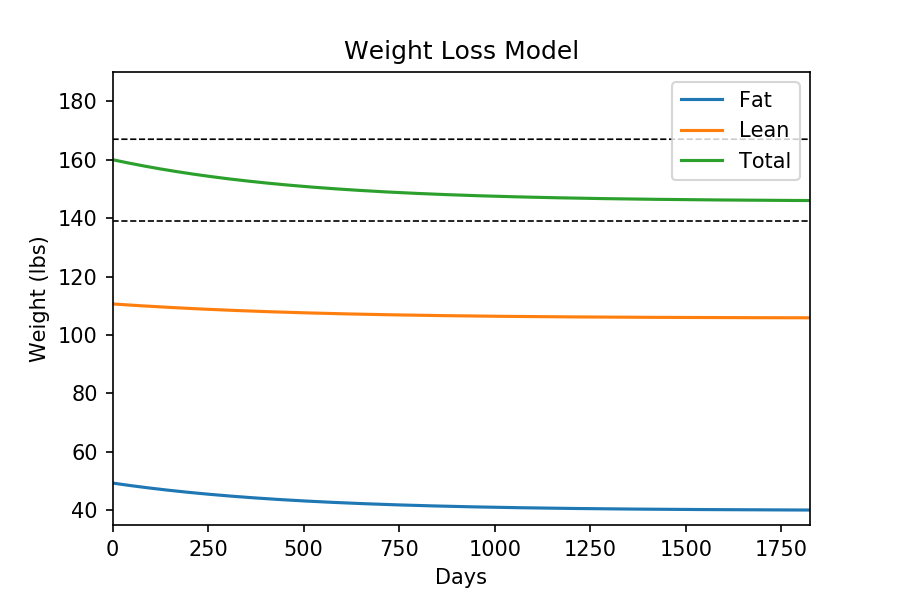
\includegraphics[width=\textwidth]{figures/weightloss_graph.png}
\caption{The solution of the weight change model for problem 6.}
\label{fig:weightloss}
\end{figure}

\begin{problem}
%Define the function \li{weight_odesystem()} as given in \eqref{eqn:compartment} using the functions \li{forbes()} and \li{energy_balance()} provided. 

Consider the initial value problem corresponding to \eqref{eqn:compartment}.
\begin{align}
	\begin{split}
\dfrac{dF(t)}{dt} &= \frac{(1-p(t)) EB(t)}{\rho_F},\\
\dfrac{dL(t)}{dt} &= \frac{p(t) EB(t)}{\rho_L},\\
F(0) &= F_0, \\
L(0) &= L_0.
	\end{split}\label{eqn:weight_prob1}
\end{align}

The following function returns the fat mass of an individual based on body weight (kg), age (years), height (meters), and sex. Use this function to define initial conditions $F_0$ and $L_0$ for the IVP above: $F_0= fat\_mass(args^*)$, $L_0 = BW - F_0$.%Using the result of this function and the provided body weight, you can define initial conditions $F_0$ and $L_0$ for the IVP above, with $F_0 =$\li{fat_mass(args^*)} and $L_0 = BW - F_0$.
\begin{lstlisting}
def fat_mass(BW, age, H, sex):
    BMI = BW / H**2.
    if sex == 'male':
        return BW * (-103.91 + 37.31 * log(BMI) + 0.14 * age) / 100
    else:
        return BW * (-102.01 + 39.96 * log(BMI) + 0.14 * age) / 100
\end{lstlisting}
%To solve this IVP for a specific individual we need initial conditions $F_0$ and $L_0.$
%The function \li{fat_mass} given earlier calculates $F_0$ based on an individual's body weight (kg), age, height (meters), and gender.
%$L_0$ is then given by $L_0 = BW - F_0$.

Suppose a 38 year old female, standing 5'8'' and weighing 160 lbs, reduces her intake from 2143 to 2025 calories/day, and increases her physical activity from little to no exercise (PAL=1.4) to exercising to 2-3 days per week (PAL=1.5).

Use \eqref{eqn:K2} and the original intake and phyical activity levels to compute $K$ for this system. Then use \li{solve_ivp} to solve the IVP. Graph the solution curve for this single-stage weightloss intervention over a period of 5 years. Your plot should match figure \ref{fig:weightloss}.
%Using \li{scipy.integrate.ode}, find and graph the solution curve for this single-stage weightloss intervention over a period of 5 years. 

Note the provided code requires quantities in metric units (kilograms, meters, days) while our graph is converted to units of pounds and days.
\end{problem}

\begin{problem}
Modify the preceding problem to handle a two stage weightloss intervention:
Suppose for the first 16 weeks intake is reduced from 2143 to 1600 calories/day and physical activity is increased from little to no exercise (PAL=1.4) to an hour of exercise 5 days per week (PAL=1.7).
The following 16 weeks intake is increased from 1600 to 2025 calories/day, and exercise is limited to only 2-3 days per week (PAL=1.5).

You will need to recompute $F_0$, and $L_0$ at the end of the first 16 weeks, but $K$ will stay the same. 
Find and graph the solution curve over the 32 week period.
\end{problem}

\begin{comment}
\section*{Variations on the Predator-Prey}
\subsection*{The Lotka-Volterra model}
Reconsider \eqref{eqn: Pred-Prey}. This representation of the predator-prey relationship is called the Lotka-Volterra predator-prey model. This well-known system of ODEs is typically given by
%This type of problem has a special name.
%The Lotka-Volterra predator-prey model is a well-known
%system of ODEs given by
\begin{align*}
	\frac{du}{dt} &= au - buv,\\
	\frac{dv}{dt} &= -cv + duv.
\end{align*}
where $u$ and $v$ represent the prey and predator populations, respectively. Here $a$ represents the rate of growth of the prey, and $bu$ the amount of prey being eaten.
Similarly, $c$ represents the rate of natural predator death, and $du$ the growth of the predator population due to the quantity of prey eaten.

Let us look at the dynamics of this system. The equlibria (fixed points) of a system occur when the derivatives are zero, for our system this occurs at $(u,v)=(0,0)$ and $(u,v)=(\frac{c}{d},\frac{a}{b})$.
%Notice also that if $v=0$ (there are no predators), the population of prey will grow exponentially.
Visualizing the phase portrait helps to give more insight into the dynamics of a system. We will do this by first nondimensionalzing our system to reduce the number of parameters.
First we note that there are exactly two equilibria (fixed points): either $(u,v) = (0,0)$ corresponding to the extinction of both species, or $(u,v) = (\frac{c}{d},\frac{a}{b})$.
Furthermore, from the ODEs we can see that if $v=0$ (there is an absence of any predators) then the population of prey will grow exponentially.

To get a better idea of the dynamics of this system we will graph its phase portrait.
We begin by nondimensionalizing the system to reduce the number of parameters:
Let $U = \frac{d}{c}u,$ $V = \frac{b}{a}v$, $\bar{t} = at,$ and $\alpha = \frac{d}{a}$.
Substituting into the original ODEs we obtain the nondimensional system of equations
\begin{align}
	\begin{split}
	\frac{dU}{d\bar{t}} &= U(1-V),\\
	\frac{dV}{d\bar{t}} &= \alpha V (U-1).
	\end{split}\label{lotka_volterra}
\end{align}
In the following code we plot the phase portrait of \eqref{lotka_volterra} along with a example trajectory, see Figures  \ref{fig:pred-prey_Lotka_Voterra} and \ref{fig:pred-prey_Lotka_Voterra_Phase_Portrait}.
We will use \li{scipy.integrate.odeint} which acts similar to the \li{ode} function used earlier but integrates over all the time steps at once.
To plot the direction field for the equations we use \li{numpy}'s \li{meshgrid} function and \li{matplotlib}'s \li{quiver} function.

\begin{figure}
\centering
\includegraphics[width=\textwidth]{Lotka_Volterra.pdf}
\caption{The solution of the nondimensionalized Lotka-Volterra predator-prey equations with parameter $\alpha = 1/3$.
This solution has initial conditions $(U,V) = (3/4, 3/4)$.}
\label{fig:pred-prey_Lotka_Voterra}
\end{figure}

\begin{lstlisting}
from scipy.integrate import odeint
a, b = 0., 13.                    # (Nondimensional) Time interval for one 'period'
alpha = 1. / 3                    # Nondimensional parameter
dim = 2                           # dimension of the system
y0 = np.array([1 / 2., 1 / 3.])   # initial conditions

# Note: swapping order of arguments to match the calling convention
# used in the built in IVP solver.
def Lotka_Volterra(y, x):
    return np.array([y[0] * (1. - y[1]), alpha * y[1] * (y[0] - 1.)])

subintervals = 200
# Using the built in ode solver
Y = odeint(Lotka_Volterra, y0, np.linspace(a, b, subintervals))

# Plot the direction field
Y1, Y2 = np.meshgrid(np.arange(0, 4.5, .2), np.arange(0, 4.5, .2), sparse=True, copy=False)
U, V = Lotka_Volterra((Y1, Y2), 0)
Q = plt.quiver(Y1[::3, ::3], Y2[::3, ::3],  U[::3, ::3],  V[::3, ::3], pivot='mid', color='b', units='dots',width=3.)
# Plot the 2 Equilibrium points
plt.plot(1, 1, 'ok', markersize=8)
plt.plot(0, 0, 'ok', markersize=8)
# Plot the solution in phase space
plt.plot(Y[:,0], Y[:,1], '-k', linewidth=2.0)
plt.plot(Y[::10,0], Y[::10,1], '*b')

plt.axis([-.5, 4.5, -.5, 4.5])
plt.title("Phase Portrait of the Lotka-Volterra Predator-Prey Model")
plt.xlabel('Prey',fontsize=15)
plt.ylabel('Predators',fontsize=15)
plt.show()
\end{lstlisting}

\begin{problem}
Compute the solutions $(U,V)$ of \eqref{lotka_volterra} 
% \begin{align*}
% 	\frac{dU}{d\bar{t}} &= U(1-V),\\
% 	\frac{dV}{d\bar{t}} &= \alpha V (U-1).
% \end{align*}
for initial conditions $(1/2, 3/4)$, $(1/16, 3/4)$, and $(1/40, 3/4)$.
Add these solutions to the phase portrait of the Lotka-Volterra model.
Can you see any limitations of this model?
\end{problem}

\begin{figure}
\centering
\includegraphics[width=\textwidth]{Lotka_Volterra_Phase_Portrait.pdf}
\caption{The phase portrait for the nondimensionalized Lotka-Volterra predator-prey equations with parameters $\alpha = 1/3$.
The portrait includes the direction field, the two equilibrium points, and the graph of the solution with initial conditions $(U,V) = (3/4, 3/4)$. }
\label{fig:pred-prey_Lotka_Voterra_Phase_Portrait}
\end{figure}

\subsection*{The Logistic model}
We have already noticed that in the absence of predators, the Lotka-Volterra equations predict that the prey population will grow exponentially.
The logistic predator-prey equations change this dynamic by adding a term to give the prey population a carrying capacity $K$:
\begin{align*}
	\frac{du}{dt} &= au\left(1 -\frac{u}{K}\right) - buv,\\
	\frac{dv}{dt} &= -cv + duv.
\end{align*}
Let $U = \frac{u}{K},$ $V = \frac{b}{a}v$, $\bar{t} = at,$  $\alpha = \frac{dK}{a}$, and $\beta = \frac{c}{dK}$.
Then the nondimensional logistic equations are
\begin{align}
	\begin{split}
	\frac{dU}{d\bar{t}} &= U(1-U-V),\\
	\frac{dV}{d\bar{t}} &= \alpha V (U-\beta).
	\end{split} \label{logistic_pred_prey}
\end{align}

\begin{problem}
Compute the solutions $(U,V)$ of \eqref{logistic_pred_prey}
for initial conditions $(1/3, 1/3)$ and $(1/2, 1/5)$.
Do this for parameter values $\alpha, \beta = 1, .3$ and also for values $\alpha, \beta = 1, 1.1$.
Create a phase portrait for the logistic equations using both sets of parameter values.
Remember to plot the direction field, all equilibrium points, and the orbits of the solutions.
\end{problem} 
\end{comment}
